\subsubsection{Ý tưởng}
\textbf{Shell Sort} là một cải tiến của thuật toán \textbf{Insertion Sort}. Ý tưởng chính là sắp xếp các phần tử nằm xa nhau trước, sau đó giảm dần khoảng cách giữa các phần tử so sánh, và cuối cùng thực hiện một lần \textbf{Insertion Sort} với các khoảng cách bằng 1. Điều này giúp giảm số lần hoán đổi và so sánh khi so sánh các phần tử gần nhau ở bước cuối.

\subsubsection{Mã giả}
\begin{algorithm}[H]
\caption{ShellSort}
\begin{algorithmic}[1]
\Procedure{\textbf{ShellSort}}{$arr, n$}
    \State \textbf{Input:} Mảng $arr$ gồm $n$ phần tử
    \State \textbf{Output:} Mảng $arr$ được sắp xếp
    \State $gap \gets n/2$
    \While {$gap > 0$}
        \For {$i \gets gap$ \textbf{to} $n - 1$} 
            \State $temp \gets arr[i]$
            \State $j \gets i$
            \While{$j \geq gap$ \textbf{and} $arr[j - gap] > temp$}
                \State $arr[j] \gets arr[j - gap]$
                \State $j \gets j - gap$
            \EndWhile
            \State $arr[j] \gets temp$
        \EndFor
        \State $gap \gets gap / 2$
    \EndWhile
\EndProcedure
\end{algorithmic}
\end{algorithm}
\subsubsection{Ví dụ}
Dưới đây là các bước chạy tay của thuật toán \textbf{Shell Sort}:
\begin{figure}[H]
    \centering
    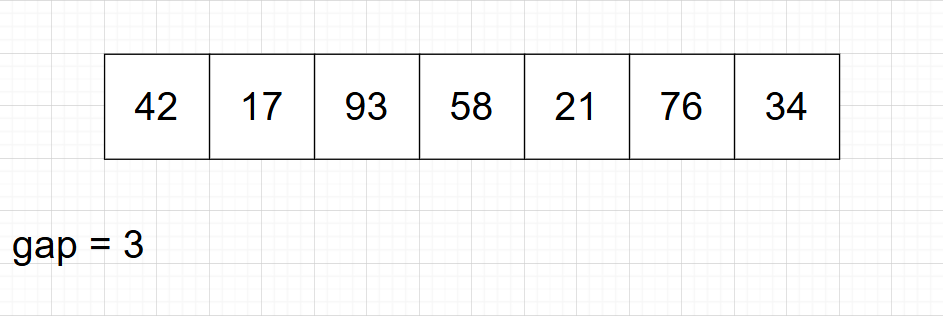
\includegraphics[width=1\linewidth]{img/shell_sort/1.png}
    \vspace{0.15cm}
    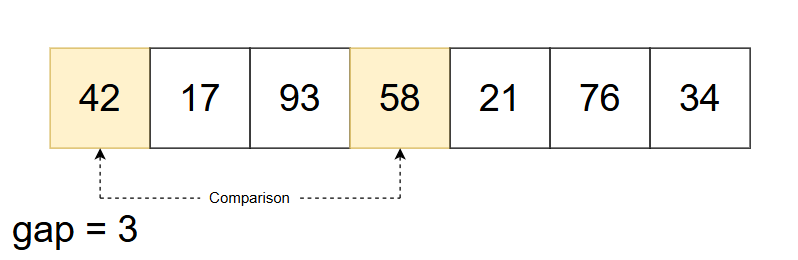
\includegraphics[width=1\linewidth]{img/shell_sort/2.png}
    \vspace{0.15cm}
    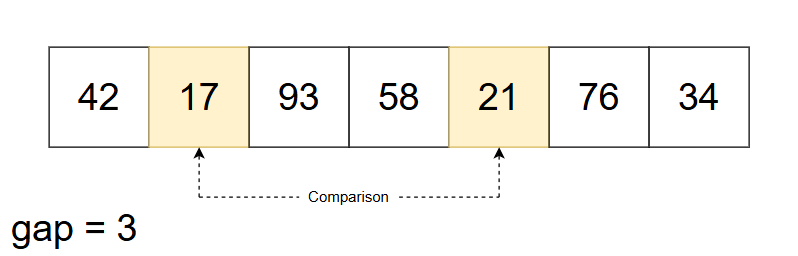
\includegraphics[width=1\linewidth]{img/shell_sort/3.png}
    \vspace{0.15cm}
    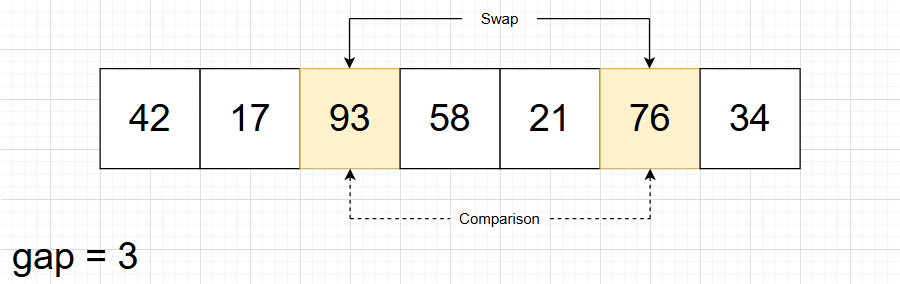
\includegraphics[width=1\linewidth]{img/shell_sort/4.png}
    \caption{Các bước chạy - 1}
    \label{fig:part1}
\end{figure}

\begin{figure}[H]
    \centering
    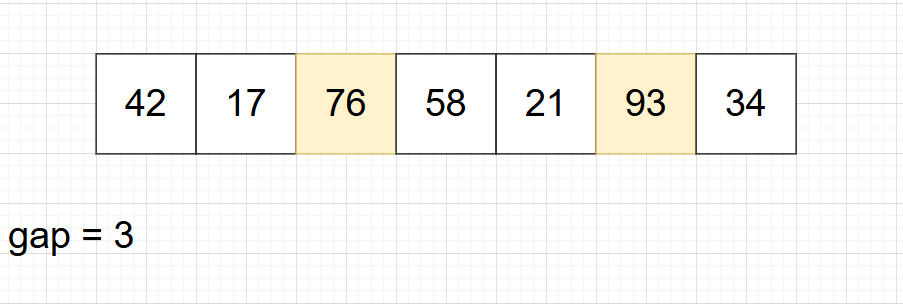
\includegraphics[width=1\linewidth]{img/shell_sort/5.png}
    \vspace{0.5cm}
    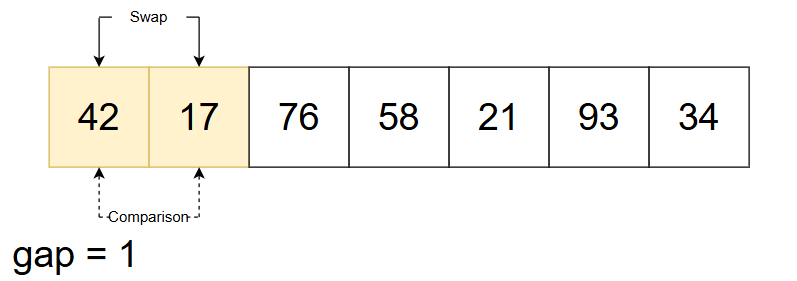
\includegraphics[width=1\linewidth]{img/shell_sort/6.png}
    \vspace{0.15cm}
    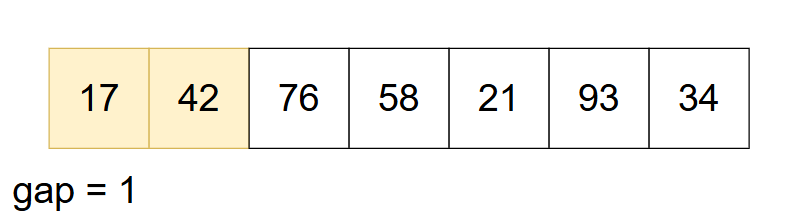
\includegraphics[width=1\linewidth]{img/shell_sort/7.png}
    \vspace{0.15cm}
    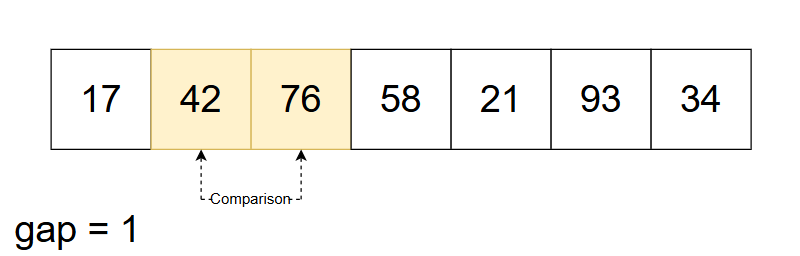
\includegraphics[width=1\linewidth]{img/shell_sort/8.png}
    \caption{Các bước chạy - 2}
    \label{fig:part2}
\end{figure}

\begin{figure}[H]
    \centering
    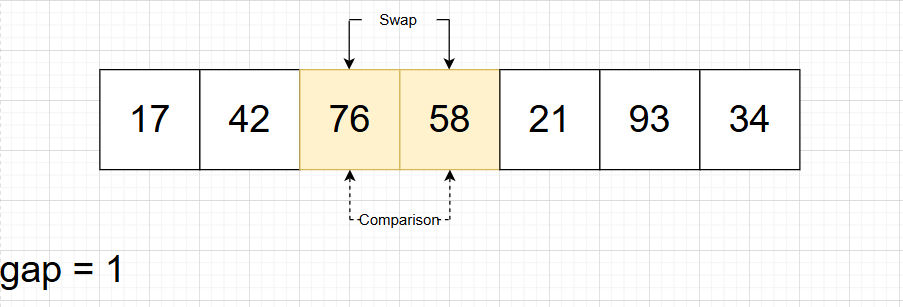
\includegraphics[width=1\linewidth]{img/shell_sort/09.png}
    \vspace{0.15cm}
    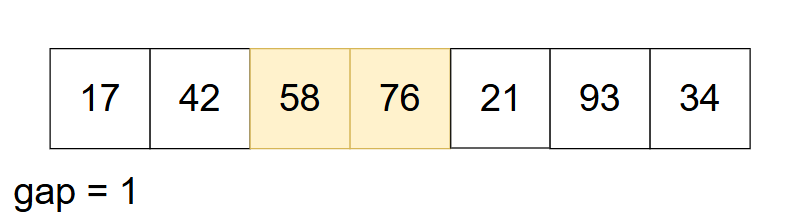
\includegraphics[width=1\linewidth]{img/shell_sort/10.png}
    \vspace{0.15cm}
    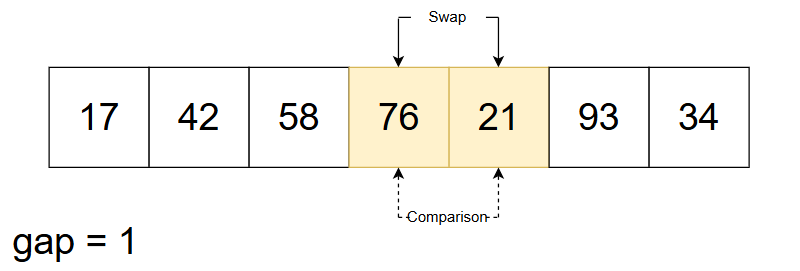
\includegraphics[width=1\linewidth]{img/shell_sort/11.png}
    \vspace{0.15cm}
    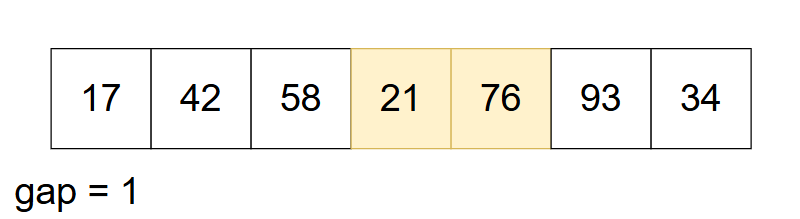
\includegraphics[width=1\linewidth]{img/shell_sort/12.png}
    \caption{Các bước chạy - 3}
    \label{fig:part3}
\end{figure}

\begin{figure}[H]
    \centering
    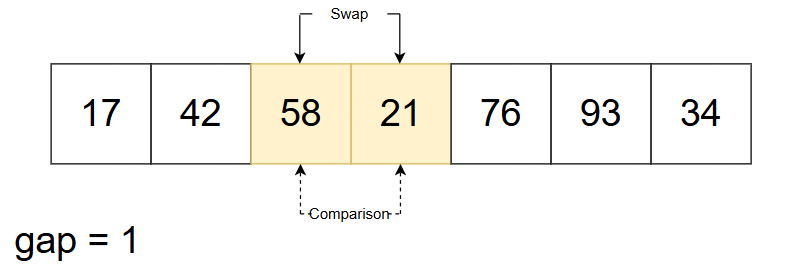
\includegraphics[width=1\linewidth]{img/shell_sort/13.png}
    \vspace{0.15cm}
    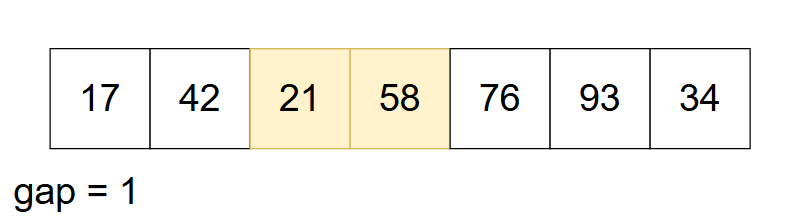
\includegraphics[width=1\linewidth]{img/shell_sort/14.png}
    \vspace{0.15cm}
    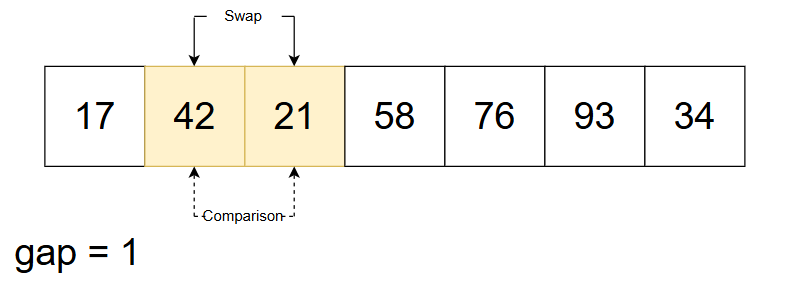
\includegraphics[width=1\linewidth]{img/shell_sort/15.png}
    \vspace{0.15cm}
    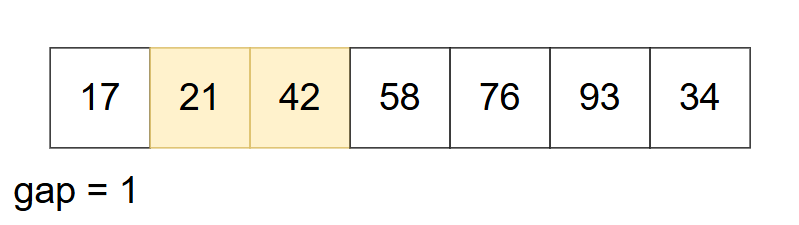
\includegraphics[width=1\linewidth]{img/shell_sort/16.png}
    \caption{Các bước chạy - 4}
    \label{fig:part4}
\end{figure}

\begin{figure}[H]
    \centering
    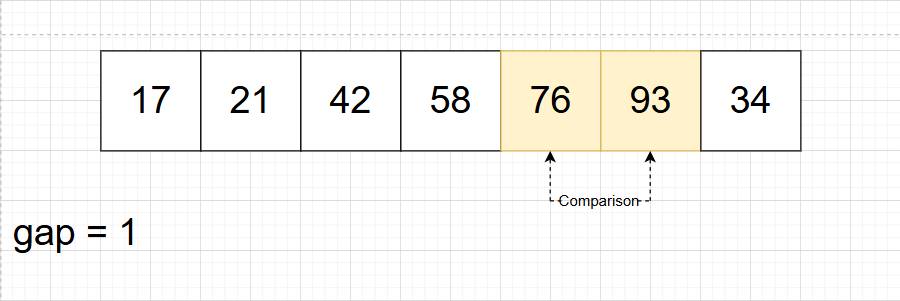
\includegraphics[width=1\linewidth]{img/shell_sort/17.png}
    \vspace{0.15cm}
    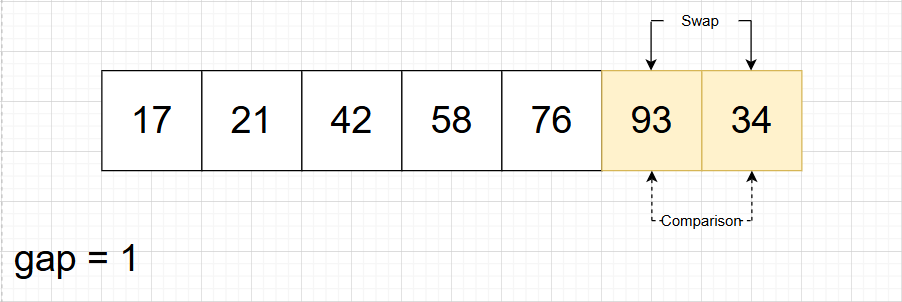
\includegraphics[width=1\linewidth]{img/shell_sort/18.png}
    \vspace{0.15cm}
    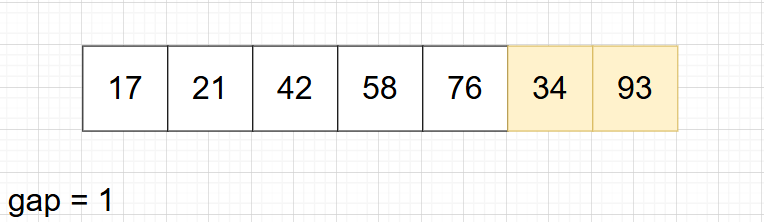
\includegraphics[width=1\linewidth]{img/shell_sort/19.png}
    \vspace{0.15cm}
    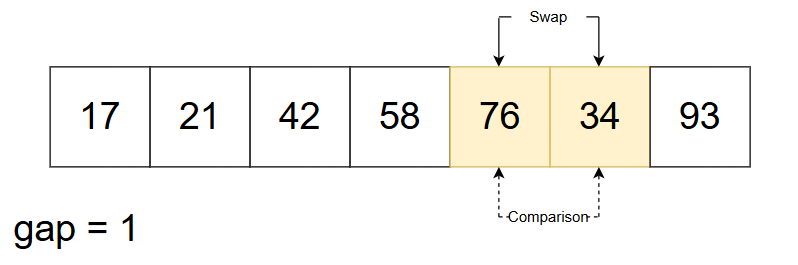
\includegraphics[width=1\linewidth]{img/shell_sort/20.png}
    \caption{Các bước chạy - 5}
    \label{fig:part5}
\end{figure}

\begin{figure}[H]
    \centering
    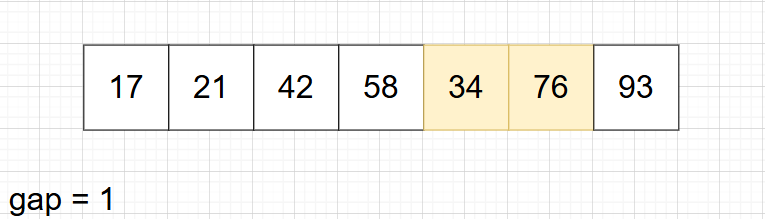
\includegraphics[width=1\linewidth]{img/shell_sort/21.png}
    \vspace{0.15mm}
    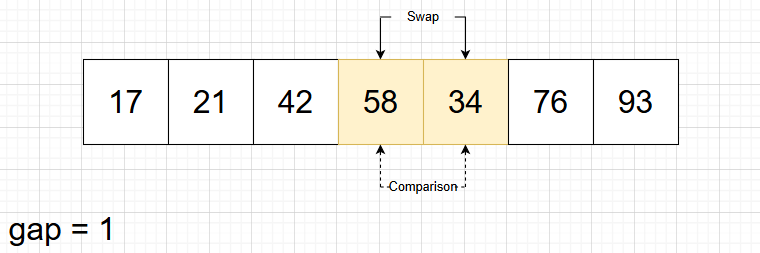
\includegraphics[width=1\linewidth]{img/shell_sort/22.png}
    \vspace{0.15mm}
    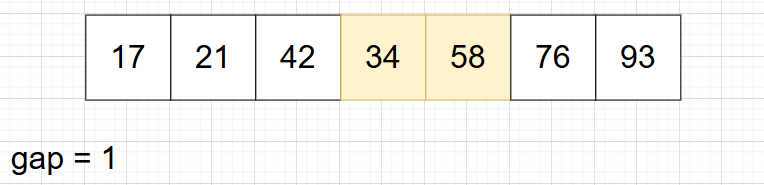
\includegraphics[width=1\linewidth]{img/shell_sort/23.png}
    \vspace{0.15mm}
    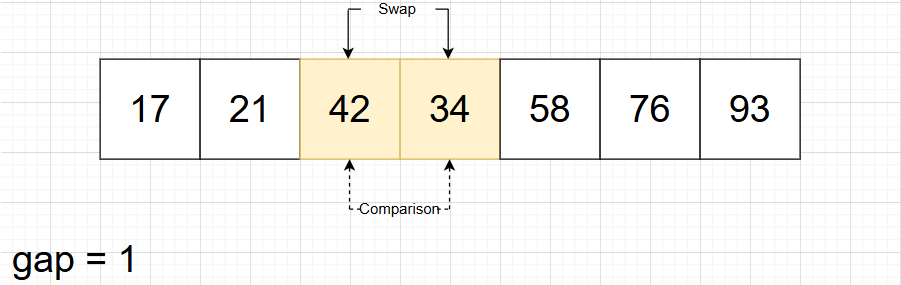
\includegraphics[width=1\linewidth]{img/shell_sort/24.png}
    \vspace{0.15mm}
    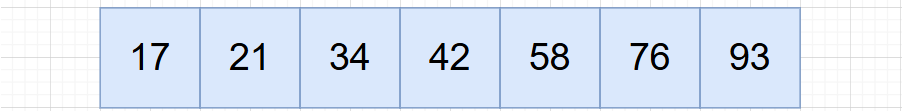
\includegraphics[width=1\linewidth]{img/shell_sort/25.png}
    \caption{Các bước chạy - 6}
    \label{fig:part6}
\end{figure}

\subsubsection{Độ phức tạp}
\begin{itemize}
    \item[\textbf{--}] \textbf{Độ phức tạp về thời gian:}
    \begin{itemize}
        \item[$\bullet$] \textbf{Best Case:} $\mathcal{O}(n \cdot \log n)$, phụ thuộc vào cách chọn chuỗi khoảng cách (gap sequence). Khi mảng gần như đã được sắp xếp, số phép hoán đổi và so sánh giảm đáng kể.
        \item[$\bullet$] \textbf{Average Case:} $\mathcal{O}(n^{3/2})$, đối với chuỗi khoảng cách phổ biến như Knuth hoặc Hibbard. Đây là độ phức tạp trung bình được quan sát trong thực tế và lý thuyết.
        \item[$\bullet$] \textbf{Worst Case:} $\mathcal{O}(n^2)$, xảy ra khi mảng có cấu trúc dữ liệu bất lợi hoặc chuỗi khoảng cách không được tối ưu hóa.
    \end{itemize}
    \item[\textbf{--}] \textbf{Độ phức tạp về không gian:} $\mathcal{O}(1)$, do thuật toán thực hiện in-place, không yêu cầu bộ nhớ phụ trợ.
    \item[\textbf{--}] \textbf{Tính ổn định:} Thuật toán không ổn định, vì trong quá trình di chuyển các phần tử qua khoảng cách lớn, thứ tự ban đầu của các phần tử có giá trị bằng nhau có thể bị thay đổi.
\end{itemize}
